\section{Idea}

gamma-sky.net is a one-stop resource for browsing images and catalogs but also for closely examining a specific gamma-ray source. Although it was mainly built for the greater astronomical community, the webpage additionally targets the general public through a user-friendly interface and a clean information layout, all of which are compiled under cutting-edge web tools.

\begin{figure}[t]
\centerline{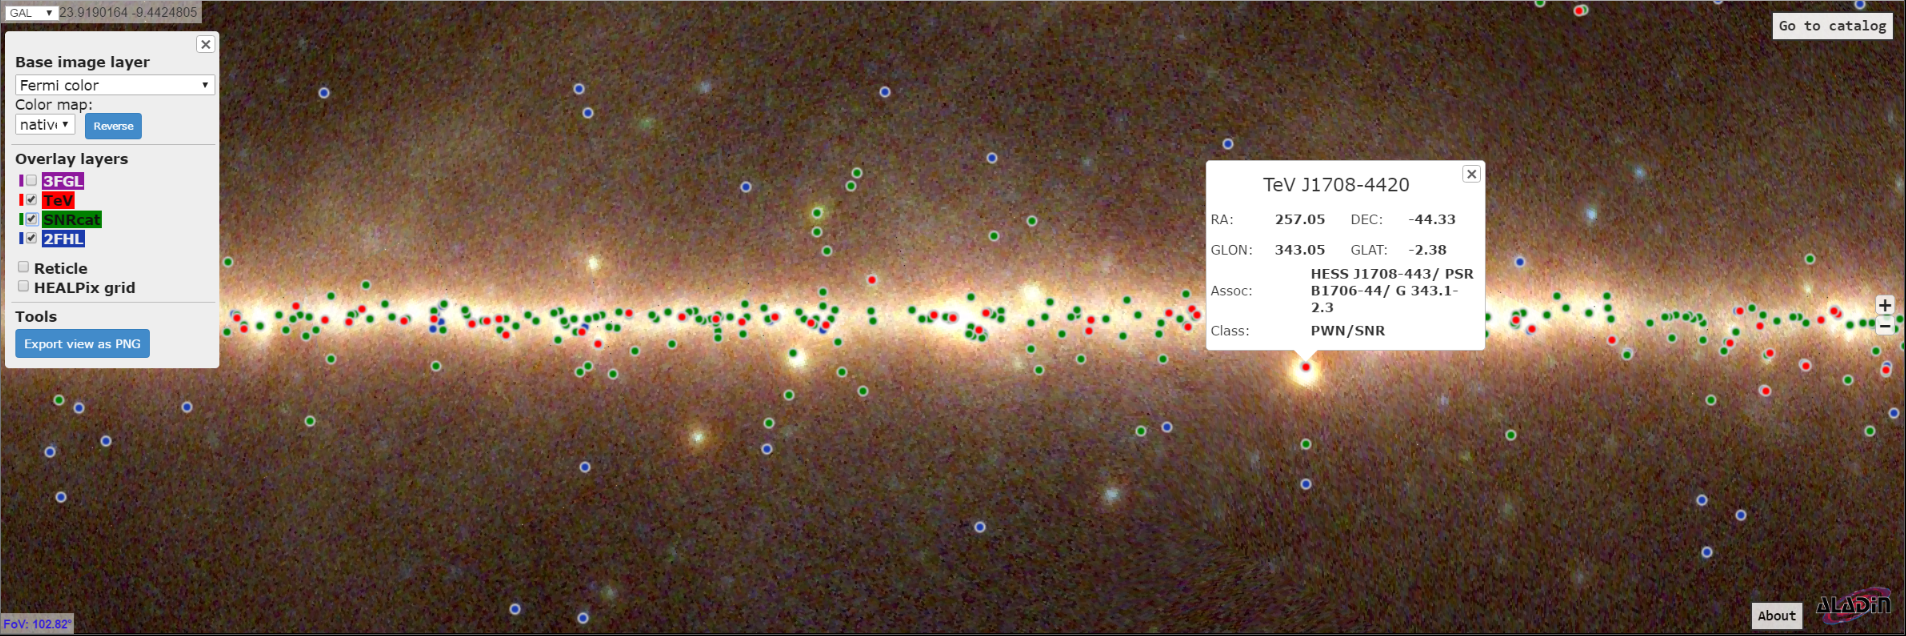
\includegraphics[width=\textwidth]{figures/mapview_wide}}
\caption{Map View.}
\label{fig:mapview}
\end{figure}

\begin{figure}[t]
\centerline{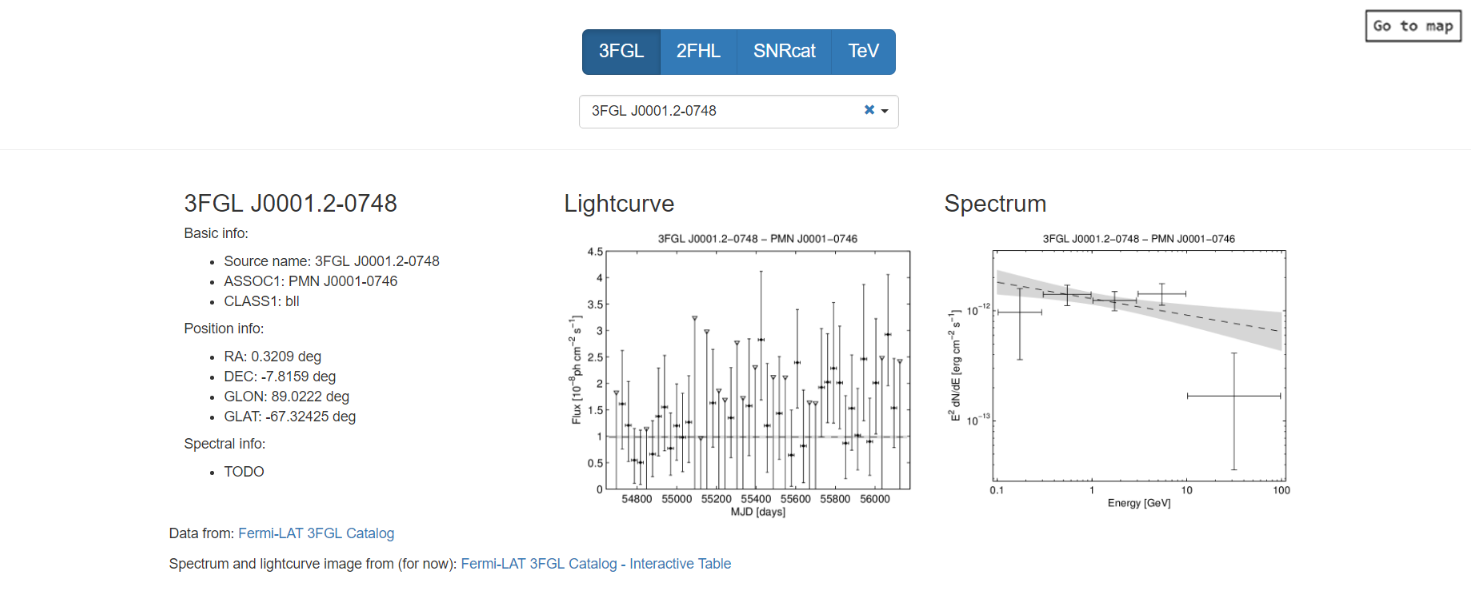
\includegraphics[width=\textwidth]{figures/catview_wide_zoom}}
\caption{Catalog View.}
\label{fig:catview}
\end{figure}

Individuals who access the website via any modern internet browser will be welcomed with the Map View page. This page presents an overlay of multi-wavelength survey images, most of which are all-sky images, wrapped around a three-dimensional sphere. The map features pan-and-zoom functionality for easily navigating and quickly browsing the sky. Gamma-ray sources from our catalog data have been pinpointed onto the sphere, as shown in Figure~\ref{fig:mapview}. The Map View page also utilizes a powerful search tool to either pan the view to a given sky position or locate a source by name. This functionality allows the user to easily find their sources and study their visual context in relation to other objects. gamma-sky.net additionally embodies a Catalog View, which incorporates more detailed information for each of the sources in our catalogs. Professional astronomers will navigate to this component of the website for the deep investigation of a particular source. See the Catalog View page in Figure~\ref{fig:catview}.

It is imperative for all of our data on the online portal to be openly available for download and local analysis by any user. Additionally, gamma-sky.net is an entirely open-source project and other developers are welcome to contribute to the code. We advise those interested in contributing to visit our GitHub repository at \url{https://github.com/gammapy/gamma-sky}.
